\chapter{Method}\label{chap:method}
This chapter will describe the work process of this project. It will describe what has been done and discuss the decisions taken.

\section{Deciding on a dataset}\label{sec:deciding_dataset}
As described in the initial problem description, deciding on a dataset is essential for the project to proceed. A first step was thus to find a dataset which satisfies the constraints presented in section \ref{sec:select_dataset}. This was needed as a first step since an artificial neural network needs a good source of data to learn from. Since using ANN is a supervised learning technique the data used to train it must be labelled. It thus saves a lot of time if the chosen dataset is already labelled when fetching it or that it can be automatically labelled by some automated process. Manually labelling several thousands of data points was never an option when deciding on the dataset. It would be too time consuming for the scope of the project.
\\\\
After searching for difference sources of data it finally came down to two datasets; Ubuntu Dialogue Corpus \parencite{lowe2015ubuntu} and Reddit data (see appendix \ref{appendix:reddit}). The Ubuntu Dialogue Corpus contained forum posts with back and forth discussions whereas the Reddit dataset contained a post and whether a certain user had up or down voted that post. Using The Reddit Application Programming Interface (API) (\url{https://www.reddit.com/dev/api/}) it was also possible to extract more information from a post, such as which subreddit it belonged to.
\\\\
The reason for having the Ubuntu Dialogue Corpus and the Reddit up-votes and down-votes data as final considerations comes down to a few factors. Most important were the overall characteristics of the data; it was text content written by users for other users. There were also interaction with the content which could be used to indicate interest in a topic. The availability of the data, its format and its size were also factors.
\\\\
After comparing the two datasets the Reddit dataset was chosen. It had a very simple format but primarily it had a very strong indication of user interest compared to the Ubuntu Dialogue Corpus. In the Reddit dataset content was directly linked to users on the platform which had either up- or down-voted it. On Reddit, up or down voting content means that the user clicks a button indicating if they like or dislike a certain post. We made an assumption that an active decision to either up- or down-vote some content would indicate interest and that a general user is less likely to engage in a full discussion (as in the Ubuntu Dialogue Corpus) compared to just clicking a button.
\\\\
An example of what an entry in the Reddit dataset looks like after post-processing is shown in table \ref{table:example_reddit_data}. The raw dataset only contained IDs to posts and subreddits which had to be converted to actual content using the Reddit API. Details on the actual gathering and post-processing of the data is described in section \ref{sec:gathering_data}.
\begin{table}[h!]
    \centering
    \begin{tabu}to 1\textwidth{ X[c] X[c] X[c] X[c] X[c] } 
        \hline
        \textbf{Title} & \textbf{Content} & \textbf{Subreddit} & \textbf{Upvotes} & \textbf{Downvotes} \\
        \hline
        \hline
        &&&& \\
        A Graph of NP-complete Problems & \textit{<empty>} & compsci & izzycat, cypherx, HattoriHanzo & \textit{<empty>}\\
        &&&& \\
        \hline
    \end{tabu}
    \caption{An example data point in the post-processed Reddit dataset showing information about a post (with no content) and which users showed interest in it.}
    \label{table:example_reddit_data}
\end{table}
\\
A question that arose was how to interpret the downvotes or lack of interaction. If a user has upvoted a post an assumption is made that the user found the post enjoyable or interesting, but it is not clear what a downvote or lack of interaction could mean. If a user has downvoted a post that could potentially mean one of two things; either the user did not like the content and does not want to see similar posts again or the user find the post interesting but does not agree with the point of view of the author. Similarly with no interaction, a user might simply not have either seen the post, has not liked it or has not cared enough to vote on it. Given time constraints, the thesis only evaluates the case with the assumption that all votes, positive or negative, represent interest in the content.

\section{Gathering data}\label{sec:gathering_data}
The Reddit dataset is not so useful in its raw form. As briefly described in section \ref{sec:deciding_dataset} the raw data only consisted of ID references. As an example, a data point in the raw dataset could look like in table \ref{table:raw_reddit_data}. This is far from how the dataset looked like after processing, shown in table \ref{table:example_reddit_data}.
\begin{table}[h!]
    \centering
    \begin{tabular}{ c c c } 
        \hline
        \textbf{Username} & \textbf{Post ID} & \textbf{Vote} \\
        \hline
        \hline
        2bornot2b & t3\_89ko9 &-1\\
        \hline
    \end{tabular}
    \caption{An example data point in the raw Reddit dataset showing that the user 2bornot2b has downvoted the post with ID t3\_89ko9.}
    \label{table:raw_reddit_data}
\end{table}
\\
In the raw form shown in table \ref{table:raw_reddit_data} the data is modelled as a relation from a specific user to a specific post. A post is also represented as a single ID instead of its title, content and subreddit. To get from the raw format to the post-processed format two steps were made.   
\\\\
Firstly the ID of a post was used to retrieve more meaningful content from the Reddit API. This included getting a posts title, subreddit and eventual content (a lot of posts only had a title with no other content). To turn a single post ID into meaningful content that could be used as training data in the project the Reddit API was used. As a post ID is only a reference in Reddit's database the API could be used to extract more information by passing the ID to it. The API specifically had an endpoint that could take one or more post IDs as input and return a list with all information available about that post. This enables the extraction of the post's title and content as well as which subreddit it belongs to. As the dataset is large it would have been ineffective to make the extraction from the post ID manually, therefore the extraction task was automated. The source code is available at \url{https://github.com/kandidat-highlights/reddit-scraper}.
\\\\
Secondly the relations of the data were re-arranged to instead model a relationship from a unique post to several users. The problem with the original format is that each data point models a single user's either up- or down-vote for a post. For the problem described in this thesis the input to the system should be a post and the output should be all users who are interested in it and this is not something that can be modelled with the original format. A format where each post is represented by a single data point was desired. The same data point would also contain all users who has up or down voted the post. The way the final format, as shown in table \ref{table:example_reddit_data}, was achieved by loading all the data into a relational database. By having the data in a relational database it was easy throughout the course of the project to extract different samples of data suitable for some experiments. As an example it could be used to split the dataset into training, validation and testing subsets.

\section{Modelling the artificial neural network}\label{sec:modelling_the_ann}
The general characteristic of the problem is that given some post, one or more users should be recommended based on their previous interest in other posts. A Reddit post in the given dataset is described by three properties; a title, some content text and a subreddit (category). This means that the ANN model should be able to use natural language as input. This property of the problem motivates the use of recurrent neural network to fully capture the input of natural language. A rough initial model was thus to have an artificial neural network with an RNN for the input (first) layer, no hidden layers and a output layer.

\subsection{A basic starting point}\label{method_basic_start_point}
For the output (last) layer each user had to be represented in a way that made it possible to compare them against each other in terms of how likely they were to be interested in a given input post. This in practice meant that the output layer should scale the output of the ANN between $(0,1)$ as this allows for interpretation as probabilities. Two activation functions which does this were considered; the softmax function (see section \ref{sec:softmax_function}) and the sigmoid (see section \ref{sec:sigmoid_function}). As the problem is to recommend one \textit{or more} users it can be seen as a multi-label classification problem, which meant that using the sigmoid activation function would likely perform better. However, as a rough starting point none of the activation functions were ruled out at that stage.
\\\\
An initial model like the one just described was implemented using the machine learning framework \textit{TensorFlow} \parencite{tensorflow2015whitepaper}. For the recurrent neural network, LSTM units were used. At first the network was also modelled to only use the post title as input since this was easier as a first step than using all the features of a post. The input layer was modelled to let one LSTM unit take one word, from the input sentence, at a time as input. The number of LSTM units was chosen by analysing the data in order to capture large amount of titles. However, it is still possible to choose any positive number of LSTM units - hence this is a hyperparameter. The words were transformed to one-hot vectors as described in section \ref{sec:rnn_nlp}. This simple initial model is visualised in figure \ref{fig:first_simple_model}.
\begin{figure}[h]
    \centering
    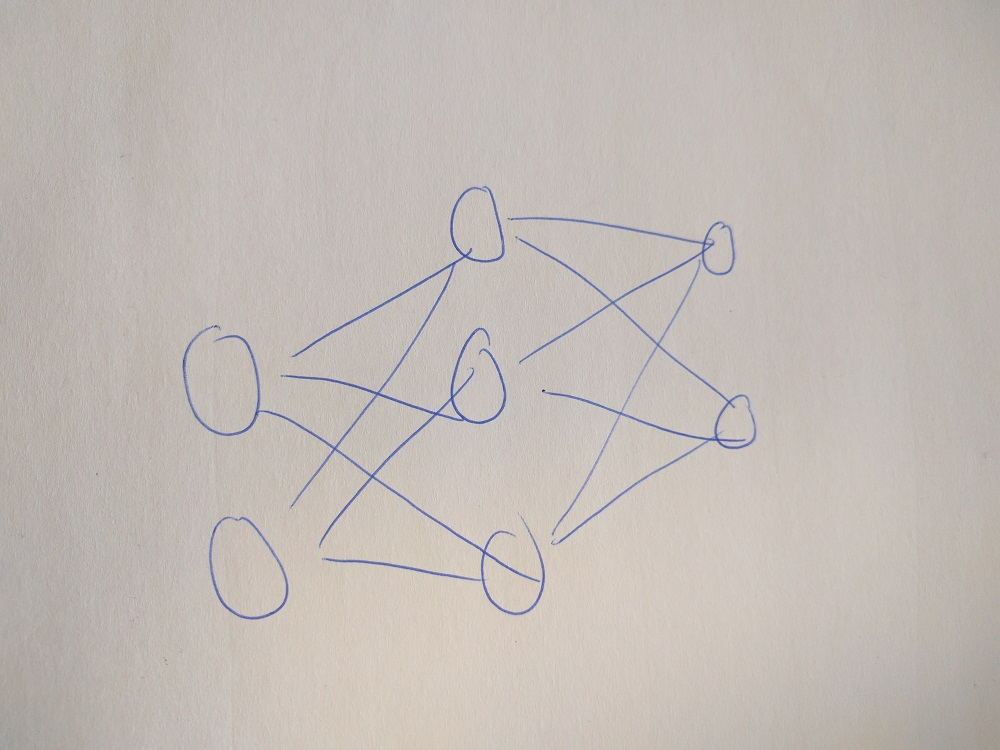
\includegraphics[width=0.75\textwidth]{figure/ann/ann}
    \caption{A graph visualisation of the first iteration model}
    \label{fig:first_simple_model}
\end{figure}
\\
A problem that quickly revealed itself was the size of the dataset. As the dataset is large, training of the network was very slow even in this simple form. A natural next step was thus to scale down the dataset to allow faster iteration of models. Instead of having a dataset with several thousands of users the dataset was downscaled into only having five users and the posts that they had interacted with. By doing the downscaling it was faster to train the network, which in turn meant that it was faster to see if it performed good or not. An assumption made using this strategy is that a model performing well on the downscaled dataset will continue to perform well as the dataset is scaled up again. 
\\\\
With this simple ANN model the goal was to establish some starting point to assure that the basic concept was working. To test that the network was actually learning anything at all we looked for overfitting (see section \ref{sec:overfitting}). If the model could not overfit on the training data using the downscaled dataset it would indicate some conceptual error or misinterpretation of the problem. However, once we had verified that the model did overfit, and thus was able to learn from the data, the work moved on to prepare a more advanced model for the actual experimentation.
\\\\
At this stage both the softmax and the sigmoid activation functions were used to test the model. With the softmax as the activation function users were picked based on a hyperparameter $k$, where $k$ was the number of users that would get predicted. This meant that the top $k$ users with the highest probabilities would always get picked as predictions from the model. In practice this meant that even if only a single user should have been predicted, the model would always predict $k$ users even if the $k-1$ remaining users shouldn't be predicted at all. The reason for using this method to pick users is based on how the softmax function normalises all probabilities. It is not practical to have a condition to pick all users with a probability higher than a certain constant, since the constant will depend on the number of users. This was however supported by the sigmoid activation function, which in the end resulted in the softmax function being removed from further testing. The limit of when to pick a user or not given a probability introduced a new hyperparameter based on how to set the limit. One option considered was to have constant limit $x$, e.g. picking all users with a probability above $x=30\%$. Choosing $x$ then becomes a problem of optimisation. Another option considered was to pick all users with an above average probability. The hyperparameter then becomes to choose which of the two options to use and to choose a value of $x$ if the first option is used.
\\\\
It is common to use $F_1$ score when evaluating machine learning models \parencite{yang1999re}. A benefit of using the sigmoid function over the softmax function was to measure more meaningful performance. The softmax function was not practical because a constant number of users would always get picked - this meant that the recall would always equal the precision. During the performance testing of the network, users were selected based on the probability that the network assigned to them if that probability exceeded a certain threshold. With the more dynamic way to predict users as the sigmoid function allowed, the recall could be calculated in a more meaningful way which in turn allowed to calculate the $F_1$ score of the model. With the sigmoid as the output function precision, recall and $F_1$ score was measured and used to evaluate the performance of the model. In order to visualise the performance a TensorFlow tool called \textit{TensorBoard} was used.
\subsection{Enhancing the model}\label{sect:enhacing_the_model}
After the performance measures were implemented to calculate precision, recall and $F_1$ score it was possible to accurately compare models against each other. Because of this, the model could now be enhanced and the changes could be evaluated. An enhancement that was easy to implement was regularisation: Both L2 regularisation and Dropout (see section \ref{sec:regularisation}) was added to the model. With regularisation two new hyperparameters were introduced; the dropout probability, $P_{dropout}$, and the L2 factor, $\beta_{L2}$. The options to use either L2 or Dropout regularisation (or both) also became hyperparameters in themselves.
\\\\
In order to add more degrees of freedom to the ANN, the model was enhanced to support hidden layers. The model was implemented so that any non-negative number of hidden layers could be used. For the layers' activation function the ReLU function was used. By adding hidden layers to the model two new hyperparameters were introduced; the number of hidden layers and how many neurons the layers should have. We simplified the model so that all hidden layers have the same number of neurons. This was to keep the number of hyperparameters, and thus the complexity, down to make experimentation easier. Each layer is connected as a chain in a fully connected way, so there are no parallel hidden layers and all nodes between the two consequent are connected. This means that the output from the RNN goes to the first hidden layer and the output from that layer then goes to the second layer and so on - until the output of the last hidden layers goes into the output layer. This is illustrated in a simplified way in figure \ref{fig:ann_hidden_layers}.
\begin{figure}[h]
    \centering
    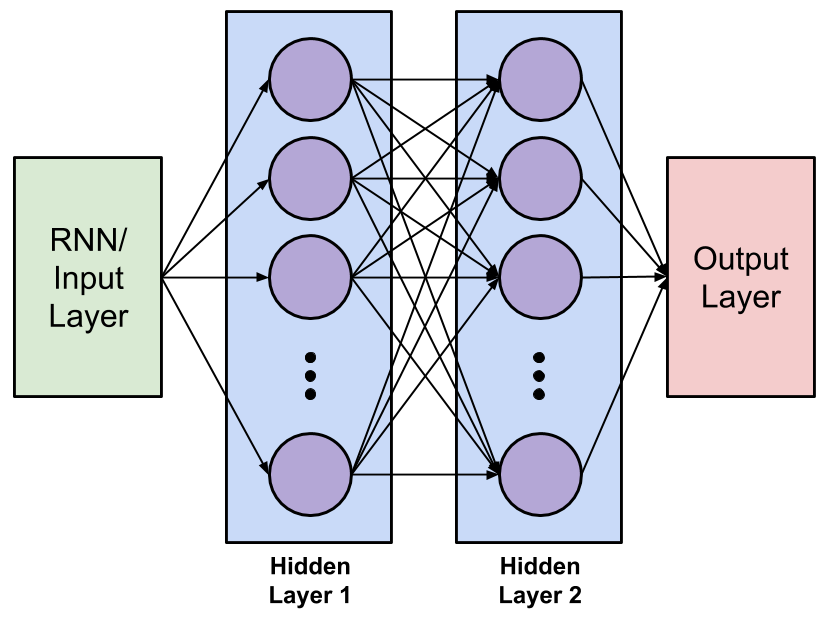
\includegraphics[width=0.75\textwidth]{figure/method/ann_hidden_layers}
    \caption{A graph visualisation of an ANN with two fully connected hidden layers.}
    \label{fig:ann_hidden_layers}
\end{figure}
\\\\
Further enhancement was to implement pre-trained word embeddings. The word embeddings would be pre-trained with GloVe \parencite{pennington2014glove}. Reason for using word embeddings is that they better capture the relation between words in a language/corpus \parencite{mikolov2013linguistic}, GloVe has also been shown to perform better compared to other methods for creating word embeddings such as word2vec \parencite{pennington2014glove}. First step is to evaluate the performance of the already pre-trained embeddings that can be found on \url{https://nlp.stanford.edu/projects/glove/}. The two specific embeddings that were evaluated are pre-trained on "Wikipedia 2014 + Gigaword 5"- and "Twitter"-datasets. During the evaluation different sizes of the embeddings would be tested to find the one that performs best on our task. Second and the last step of word embeddings is to pre-train a word embedding based on the Reddit dataset that was chosen. 
The reason for creating new embeddings is that some words can be community- or platform-specific meaning that there is a chance of capturing more relations between the words. Different dimensions of the embedding matrices will be evaluated against each other. 
\\\\
So far only the title of a post is used as input to the model. Since there is more data available about each post, such as its content and which subreddit it belongs to, the model was also enhanced to incorporate this. For the subreddits, the actual meaning of the subreddit (i.e. the actual text, e.g. \textit{politics} or \textit{humor}) was not of interest. Instead a post's subreddit was encoded as a one hot vector. This vector was fed through a linear layer and concatenated directly with the output from the existing RNN as a means to re-size its dimensions. The option to either use this extra input or not turned into another hyperparameter.
\\\\
Early in the project subreddits were tested as a classification target instead of users. The network showed good results for predicting which subreddit the post had been posted in. This led us to believe that it could be useful to first train network at predicting subreddits and then use the weights from this network as initial weights when training on users. The reasoning behind this intuition was that users probably often like posts that are in the same subreddit. If the network is then already trained to distinguish between posts in a broad term (i.e. in terms of which subreddit they belong to) that could potentially be a good starting point for distinguishing between users' interest. Combining this strategy with using both the title and subreddit of a post as input as previously mentioned was also evaluated.

\subsection{Tuning hyperparameters}
With the implementation of the model being complete, experimentation and tuning of the introduced hyperparameters was the next step. Hyperparameters are both actual parameters introduced as well as whether to use a certain feature of the model or not. For example, a model with L2 regularisation turned off is different from one with it turned on - it is also not certain that the model will perform better with it turned on. All of the hyperparameters introduced are described in table \ref{table:hyperparameters}.
\begin{table}[h!]
    \centering
    \begin{tabular}{ r  p{7cm} }
        \hline
        \textbf{Hyperparameter}  &  \textbf{Description} \\ \hline \hline
        Learning rate & A real valued number scaling the networks parameters gradients during training  \\ \hline
        Batch Size & Positive Integer specifying the size of each batch \\ \hline
        RNN units & Positive Integer specifying the number of units in the RNN  \\ \hline
        Embedding Size & todo \\ \hline
        Pre-trained embedding matrix & todo \\ \hline
        Trainable embedding matrix & A binary choice to either allow or disallow the embedding matrix to be updated during training \\ \hline
        Hidden layers & Non-negative integer specifying the number of hidden layers in the model \\ \hline
        Neurons in hidden layers & Positive Integer specifying how many neurons a particular layer has \\ \hline
        Use L2 regularisation & A binary choice to either use L2 regularisation or not \\ \hline
        L2 Factor & A real valued scaling factor for the L2 regularisation \\ \hline
        Dropout regularisation& Regularisation technique where some neuron, sometimes are deactivated \\ \hline
        Dropout probability & The probability that any given neuron will be turned off \\ \hline
        Use constant prediction limit & A binary choice to either use a constant or average based prediction limit \\ \hline
        Constant prediction limit & A threshold such that it if it surpassed a recommendation is issued  \\ \hline
        Use subreddit input & A binary choice to either use or not use the given posts subreddit as additional input \\ \hline
    \end{tabular}
    \caption{Table of all hyperparameters present in our model along with a description for each}
    \label{table:hyperparameters}
\end{table}
\\
As there are a lot of different combinations of hyperparameters a dynamic and configuration based model was implemented. With this implementation the whole model can be defined using a single configuration file. The configuration file specifies all of the hyperparameters and when the model is run it dynamically builds a computation graph to match them. This setup also enabled scheduling the training and logging the progress of different models in an automated way which made experimentation easier.
\\\\
The goal of the tuning of the hyperparameters was to maximise the $F_1$ score. Under normal circumstances an optimiser would likely be used to find the optimal parameters that maximised the $F_1$ score, but since the model is in fact an artificial neural network the time it takes for training the model makes an optimiser impractical. Instead the optimisation relies on systematic testing of different combinations of hyperparameters in an informed way. Different sets of hyperparamaters were randomly generated within some bounds. This has been proven empirically as well as theoretically to give better results instead of doing exhaustive search over all possible combinations. \parencite{bergstra2012random}
\\\\
The typical workflow when optimising the model is thus to look at previous model that had performed well, identify a hyperparameter that should be changed, test the network with the updated hyperparameter and lastly compare the results. Which hyperparameter that should be changed could be chosen on a few different bases. For example, with the boolean hyperparameters (i.e. use dropout or not) it is easy to make sure both combinations are tested and if one hasn't been tested it is a good hyperparameter to pick.
\subsection{Scaling up}
After an optimal model was found for the downscaled dataset it was time to scale up and evaluate it on a larger dataset with more users. The count of 50 users was selected for the upscaled model. 
\section{Comparing against a baseline}
When deciding how well a model performs it is compared against a baseline. The baseline puts the accuracy of the model into some context and shows how it measures up against other models. In order to have a fair comparison, the users selected are chosen in the similar way as for ANN-model mentioned in \ref{method_basic_start_point}. 
\subsection{Random classifier}
A random classifier is a model that given an input $x$ selects one of $n$ output values uniformly at random. This results in an expected accuracy of $\frac{1}{n}$. This is a baseline that any real life model needs to beat with confidence.

\subsection{N-grams based model as a baseline}
In this project a model based on n-grams \parencite{cavnar1994n} have been used as a baseline. This N-gram based model first compute  all 1, 2, and 3 -grams in the corpus and for each N-gram $g$, give it a unique number $g_i$ between $0$ and $k$ where $k$ is the total number grams in the corpus. A so called category vector is then built for each user. A category vector for user $u$, $\vec{V_u}$ is a $k$-dimensional vector with entry $\vec{V_{ui}} = n \iff $ the gram $g_i$ occurs $n$ times in the corpus for user $u$. The corpus for user $u$ is defined as all titles labelled with user $u$. Once all the category vectors have been computed the system can start making predictions. Given a new title, it is first translated into a title vector $\vec{V'}$ in a similar fashion as for the category vector, the only difference is that the corpus is limited to the title itself. Now $\vec{V'}$ is compared against all the different category vectors $\vec{V}$ using two different metrics, cosine similarity \parencite{steinbach2000comparison} and euclidean distance. The goal with using both cosine similarity and euclidean distance as metrics is that they measure different things. Cosine similarity is based on orientation while euclidean distance is based on magnitude. Which users to select is based on the chosen measurement that exceeds the mean measurement.

\subsection{Facebook fastText as a baseline}
Facebook has implemented an efficient sentence classifier called \textit{fastText} (\url{https://github.com/facebookresearch/fastText}). They used the new bag of words techniques mentioned in \parencite{joulin2016bag} in order to speed up the training since the goal of their classifier is the speed of training, making it extremely easy to run on a laptop. 
\\\\
The classifier takes in a column of sentences and a column of labels. As previously mentioned our problem can be translated so it fits facebooks classifier. More specifically, the input are titles and labels are users. \\\\
The aim is to achieve similar if not better results in terms of accuracy compared with fastText.  FastText only allows choosing top $k$ users for the performance measure. In order to compare it to the ANN model, the best F1-score was chosen from $n$ runs of performance testing. Each run chooses top $m$ users where $m$ is ranging from $1$ to $n$. The best F1-score from fastText is then compared to the F1-score of the network model.
The speed performance will be not be compared.
%Saker som man är också intressanta: Kolla upp variansen, debugg, hur vi hitta felet etc. 